\documentclass{article}
\usepackage[utf8]{inputenc}
\usepackage[margin=3cm]{geometry}
\usepackage{mathtools}
\DeclarePairedDelimiter{\ceil}{\lceil}{\rceil}
\usepackage{amsfonts} 
\usepackage{caption}
\usepackage{subcaption}
\usepackage{float}
\usepackage{titlesec}
\setcounter{secnumdepth}{5}
\usepackage{url}
\usepackage{xcolor}


\title{Master Thesis\\Machine Learning For EMG Data}
\author{Martin Colot}
\date{2021}

\begin{document}

\maketitle


\part{Introduction}


\part{State of the art}



\subsection{EMG}

\begin{itemize}
    \item What is an EMG signal
    \item EMG and EEG
    \item EMG and ENG \\
    https://pubmed.ncbi.nlm.nih.gov/33091891/  \\
    https://pubmed.ncbi.nlm.nih.gov/29498358/
    \item sEMG and iEMG sensor
    \item high density EMG \\
    https://www.sciencedirect.com/science/article/abs/pii/S1746809419302186 \\
    https://pubmed.ncbi.nlm.nih.gov/22180516/
\end{itemize}


\subsection{Myoelectric hand prosthesis}

\begin{itemize}
    \item Purpose
    \item Existing brands \\
    https://ieeexplore.ieee.org/document/8733629 \\
    https://app.dimensions.ai/details/publication/pub.1112252996?and\_facet\_journal=jour.1041772
    \item Difficulties
    \begin{itemize}
        \item limitation of non-invasive sensor
        \item Lack of EMG data for amputees
        \item Mirrored billateral training \\
        https://pubmed.ncbi.nlm.nih.gov/22180516/ \\
        https://pubmed.ncbi.nlm.nih.gov/22006428/
    \end{itemize}
\end{itemize}


\subsection{Hand gesture prediction}

\begin{itemize}
    \item Applications (prosthetic, VR)
    \item Classification and regression
\end{itemize}

\subsubsection{Preprocessing and feature selection}

\subsubsection{Gesture classification}

\begin{itemize}
    \item Classification techniques \\
    https://journals.physiology.org/doi/pdf/10.1152/jn.00555.2014 \\
    https://www.nature.com/articles/s41551-016-0025
    \item Limitations
\end{itemize}


\subsubsection{Movement regression (joint angle classification)}

\begin{itemize}
    \item Needed for a more natural feeling
    \item 27 degrees of freedom of the hand
    \item Regression techniques \\
    https://jneuroengrehab.biomedcentral.com/articles/10.1186/1743-0003-11-122 \\
    https://www.hindawi.com/journals/isrn/2012/604314/ \\
    https://pubmed.ncbi.nlm.nih.gov/22180516/
\end{itemize}





\section{Existing data set of synchronized EMG and hand gesture data}

Most of the current work concerning hand gesture prediction from sEMG signal is concentrated on gesutre classification. That is why data sets containing simultaneously sEMG signals and fingers kinematics, in the aim of doing gesture regression, are not so numerous. Moreover, there exist no state of the art benchmark for the data collection protocol which could enable to easily create such data sets.

%[TODO] show data sets made for gesture classification here

We present, in this section, two data sets containing synchronized sEMG signals and hand kinematics \cite{ref:ninapro, ref:KinMusUji} as well as some studies presenting their protocol for such data collection (without providing their data set) \cite{ref:Ngeo2014, ref:Hioki2012}.


\paragraph{Estimation of Finger Joint Angles from sEMG Using a Neural Network Including Time Delay Factor and Recurrent Structure \cite{ref:Hioki2012}}

This study was published in 2012 in the ISRN Rehabilitation journal. It uses 4 sEMG electrodes on the flexion side of the forearm with location determined by palpation. The finger joint angles were estimated using a CyberGlove. The gestures performed are based only on single finger flexion and extension and whole hand flexion and extension.

\paragraph{The NinaPro data set \cite{ref:ninapro}}

Published in 2014 in \textit{Nature Scientific Data}, this data set is composed of data acquired from 67 intact subjects and 11 who had 1 missing arm (in the aim of using the data set for hand prosthesis control). These subjects were asked to perform 4 kinds of exercises for a total of 61 different gestures (plus the resting gesture). The researchers used 12 sEMG electrodes and a CyberGlove II to estimate the hand kinematics.

This data set has been cited in multiple similar works \cite{ref:KinMusUji, ref:comp6EMGsetup}. It is however not perfect. The KIN-MUS UJI data set (presented below) shows three weaknesses that need to be corrected in order to create a reliable and reproducible benchmark.
\begin{enumerate}
    \item The performed gestures do not correspond to real life movements (ADL)
    \item The representation of the hand kinematics data is not representing anatomical angles
    \item No indication on the exact sEMG location
\end{enumerate}



\paragraph{Continuous and simultaneous estimation of finger kinematics using inputs from an EMG-to-muscle activation model \cite{ref:Ngeo2014}}

This study presents a data collection protocol together with a comparison of different prediction algorithm that make regression of the finger kinematics. The data is composed of 8 sEMG channel (each targeting a different muscle of the forearm) and finger kinematics based on a 3D motion camera system that tracks the positions of multiple markers. This technique of motion tracking is criticized by the researchers doing the KIN-MUS UJI data set for being sometimes not enough precise. 

\paragraph{The KIN-MUS UJI data set \cite{ref:KinMusUji}}

Also published in \textit{Nature Scientific Data} but in 2019, this data set aims at correcting weaknesses of the \textit{NinaPro} data set and other previews data collection protocols. In particular, it gives more precise informations on the sEMG sensor locations, its gestures are based on ALD and the hand kinematics are represented using a standardisation of the anatomical angles of the hand given by the International Society of Biomechanics (ISB) \cite{ref:handAnatomicalAngles}. The motion tracking technology used is also a CyberGlove II.


\subsection{Motion capture technologies \label{sec:motionCaptureTech}}

In order to train a regression model of the hand kinematics based on EMG signal, we need to provide a ground truth describing the evolution of the hand gesture synchronized with this signal.
Two kinds of devices are usually used to record this information: a CyberGlove or a camera motion tracking system. 

\subsubsection{CyberGlove}

The CyberGlove made by the company CyberGlove Systems (\url{http://www.cyberglovesystems.com/}) is a motion capture device composed of a glove with multiple strain gauges which capture the motion of the hand. Its latest currently available version, the CyberGlove III, can capture up to 22 joint-angles with a resolution lower than 1 degree. The  CyberGlove II was used for the creation of the Ninapro datasets \cite{ref:ninapro, ref:comp6EMGsetup} and the KIN-MUS UJI Dataset \cite{ref:KinMusUji}.

\begin{figure}[h]
    \centering
    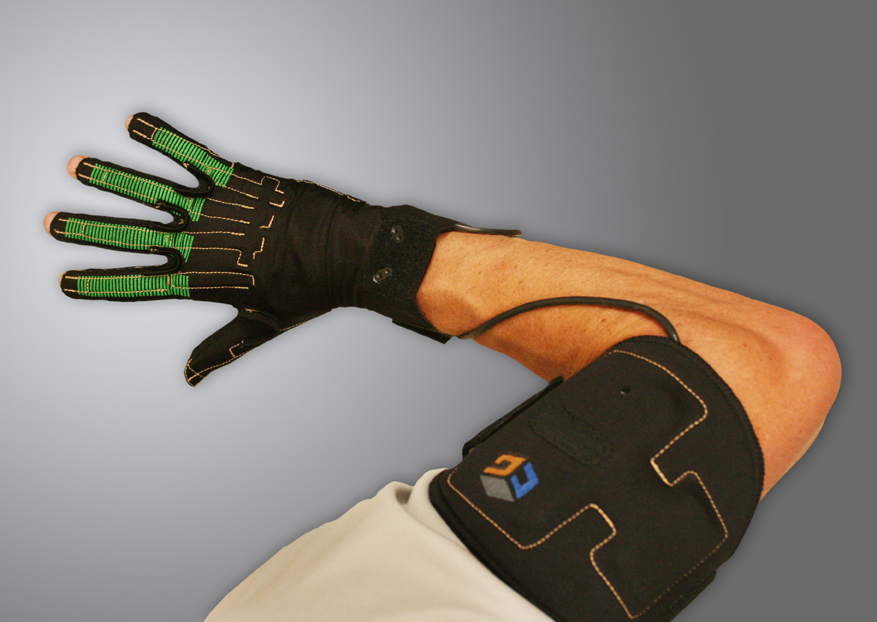
\includegraphics[width=10cm]{images/cyberGlove3.png}
    \caption{Picture of the CyberGlove III from the CyberGlove System website (\url{http://www.cyberglovesystems.com/cyberglove-iii/})}
    \label{fig:cyberGlove3}
\end{figure}

Even if this device is really easy to use and provides an accurate reconstruction of the hand joint-angles, it does not allow to easily reproduce the data collection experiment as its price can quickly reach several tens of thousands of euros and it is not easily found in every laboratory. Some people have shared instructions on how to build an homemade CyberGlove for 40 dollars \cite{ref:diyCyberGlove} but there is no guarantee on the performance that it can provide.


\subsubsection{3D motion camera tracking}

This technique is usually used for cinematographic special effects. It is composed of 2 elements: an ensemble of markers placed on the tracked object (consisting of small white balls) and a set of fixed cameras located around the subject that each film it from a different point of view. The location of each marker in the 3D space can be computed from its position each cameras vision.

To record the finger kinematics, 22 markers need to be placed as shown in the following figure.

\begin{figure}[h]
    \centering
    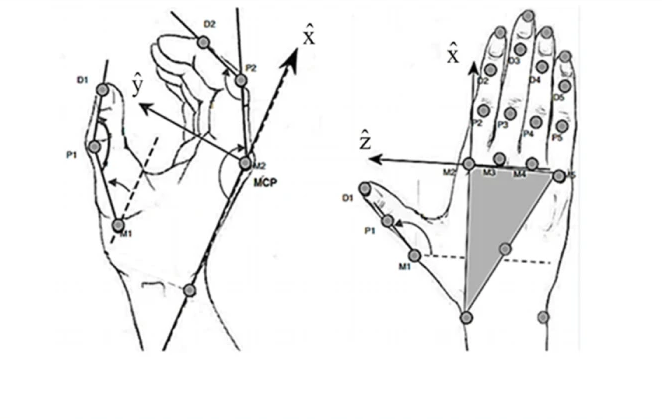
\includegraphics[width=10cm]{images/motionCaptureMarker.png}
    \caption{Positions of the 22 markers used to track the fingers kinematics \cite{ref:Ngeo2014}}
    \label{fig:cyberGlove3}
\end{figure}

This device has a precision of less than 0.5mm \cite{ref:Ngeo2014}. However, some study say that it is not reliable enough for finger tracking as their movement is too precise \cite{ref:KinMusUji}.




\subsection{sEMG Electrodes placement}

\subsubsection{Muscular activity zone identification by palpation}

When the number of available sEMG electrodes is low, studies have chosen to determine the location of these by palpation. To do this, they first need to determine a set of muscles that they want to measure \cite{ref:Hioki2012} or a set of gesture that must be recognized \cite{ref:Ngeo2014, ref:comp6EMGsetup}. Then, by performing different hand gestures, the zones with the most muscular activities are found by palpation and the electrodes placed at these locations. Visual inspection of the signal given by the electrodes can also by used to find the best spots \cite{ref:Ngeo2014}.

Even if this technique seems easy to use, it is giving poor precision on the exact spots of the electrodes which does not enable to create a reproducible data collection benchmark.


\subsubsection{Pre-identified zones giving all the muscular activity of the forearm}

A study from 2018 \cite{ref:identifiedEMGlocation} aimed at determining which zones of the forearm where sufficient to get all the muscular activity of the arm using sEMG electrodes during activities of daily living (ALD) \cite{ref:ADL1}. It started by determining 30 activity spots on the forearm, distributed on a simple grid as shown in figure \ref{fig:forearmActivityZones}.

\begin{figure}[H]
    \centering
    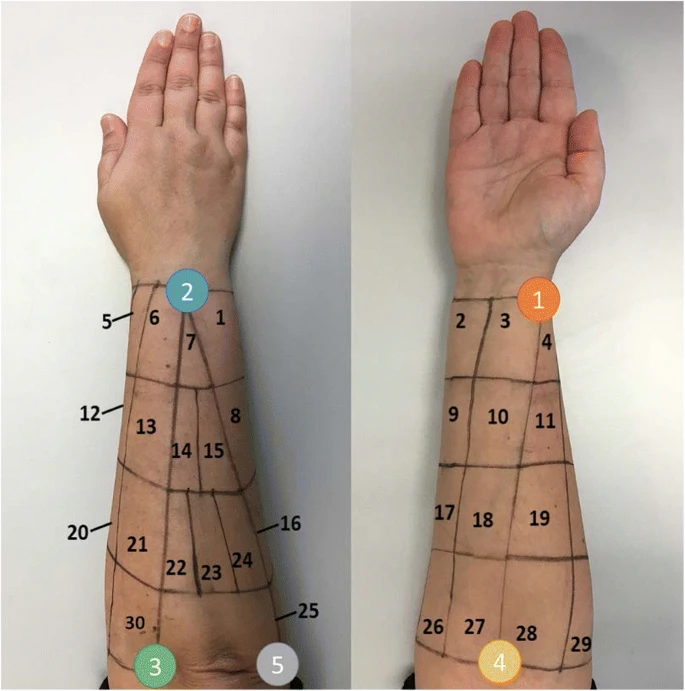
\includegraphics[width=10cm]{images/forearmActivityZones.png}
    \caption{30 spots of muscular activity on the forearm distributed on a grid \cite{ref:identifiedEMGlocation}}
    \label{fig:forearmActivityZones}
\end{figure}

The researchers recorded 21 ADL (5 sessions of 2 repetition per ADL) on 6 subjects for all 30 spots which gave them 37080 signals of 1000 temporary data which they converted into 30 function of 126000 data. Using functional principal component analysis (FPCA), they simplified the data into a set of 17 reduced variables (RV) responsible for 91\% of the muscular activity. Then, using hierarchical clustering analysis on these 17 RVs, they created a dendrogram, shown in figure \ref{fig:dendrogram}, which allowed them to determine 7 groups of spots with similar muscle activity. Finally, to choose a representative spot of each of the 7 groups, they provide the root mean square of the muscular activity of each spot (figure \ref{fig:MRS}).

\begin{figure}[H] 
\centering
\begin{subfigure}{.45 \textwidth}
    \centering
    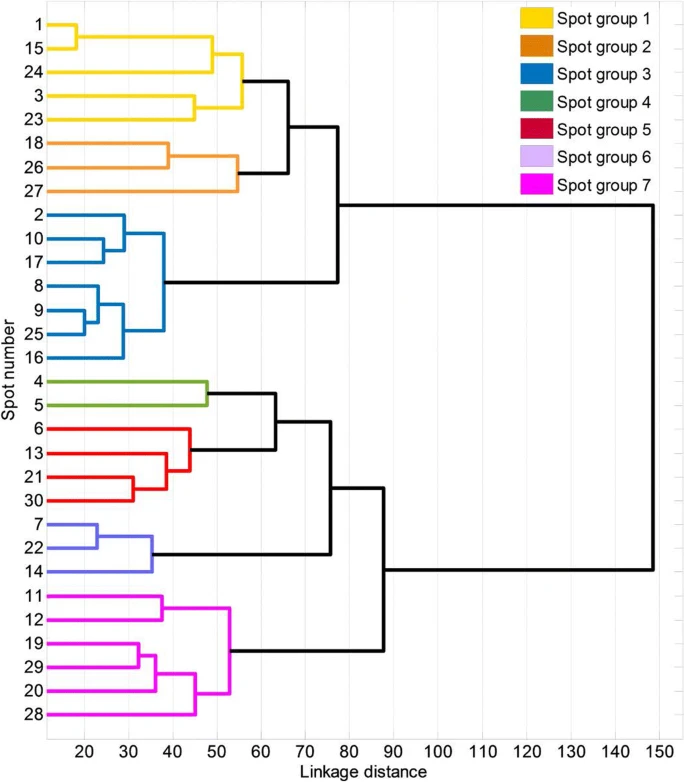
\includegraphics[width=1\linewidth]{images/forearmActivityZonesDendrogram.png}
    \caption{Dendrogram of the 30 activities zones found from hierarchical clustering analysis showing the 7 groups in different colours}
    \label{fig:dendrogram}
\end{subfigure}%
\begin{subfigure}{.45 \textwidth}
    \centering
    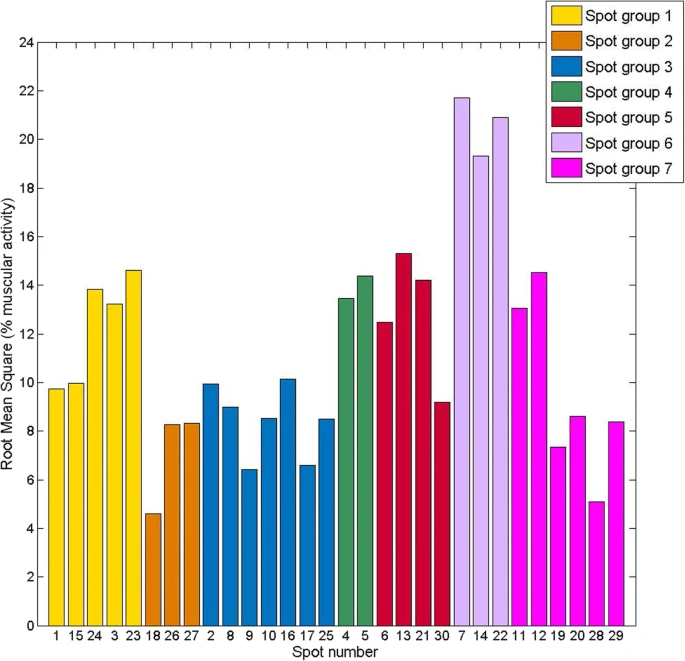
\includegraphics[width=1\linewidth]{images/forearmActivityZonesRMS.png}
    \caption{Root Mean Square of the muscular activities of the 30 activities zones showing the 7 groups in different colours}
\label{fig:MRS}
\end{subfigure}
\caption{Result of the feature selection from the 30 spots of muscular activities on the forearm during activities of daily living \cite{ref:identifiedEMGlocation}}
\end{figure}

Using this result, we can say that the best 7 spots to place sEMG sensor would be the spots 23, 27, 16, 5, 13, 7 and 12 (ordered by their group number). However, in some circumstances (muscle rehabilitation, ease of placing the electrode), other combination could be considered (as it is the case in the KIN-MUS UJI data set \cite{ref:KinMusUji}).

This method of positioning of the sensors is good for reliability and reproducibility of the data acquisition protocol. However, for a real life application of the hand kinematic prediction (i.e. for a hand myoelectric prosthesis), it might not give a practicable set of locations as they would be really sparse on the whole forearm.


\subsubsection{Myoelectric arm band}

The Myoelectric \cite{ref:myoArmBand} arm band was first developed by the company \textit{Thalmic labs}, later rebranded as \textit{North}, after having sold the patents to \textit{CTRL-labs}, a company which was later bought by \textit{Facebook} (\url{https://www.zdnet.com/article/facebook-acquires-ctrl-labs-in-machine-mind-control-research-push/}). It is a device composed of a wristband containing 8 sEMG electrodes (figure \ref{fig:myoArmband}). The main advantages are its price (only 199\$), its ease of use and the fact that it is practicable for real life application such as hand prosthesis control. On the other side, we cannot asses that the location of the sensors is always the same and that they get all the muscular activity needed to accurately predict the hand gestures.

Some studies have used this technologies to do hand gesture classification \cite{ref:Zhang2019} or to use it as an person authentication device \cite{ref:electronics9122143}. Their results were satisfying but the task that had to be done was way simpler than finger joint angles regression. As an example, the study \cite{ref:Zhang2019} only considered 5 different gestures to get a prediction accuracy of 98.7\%.


\begin{figure}[H]
    \centering
    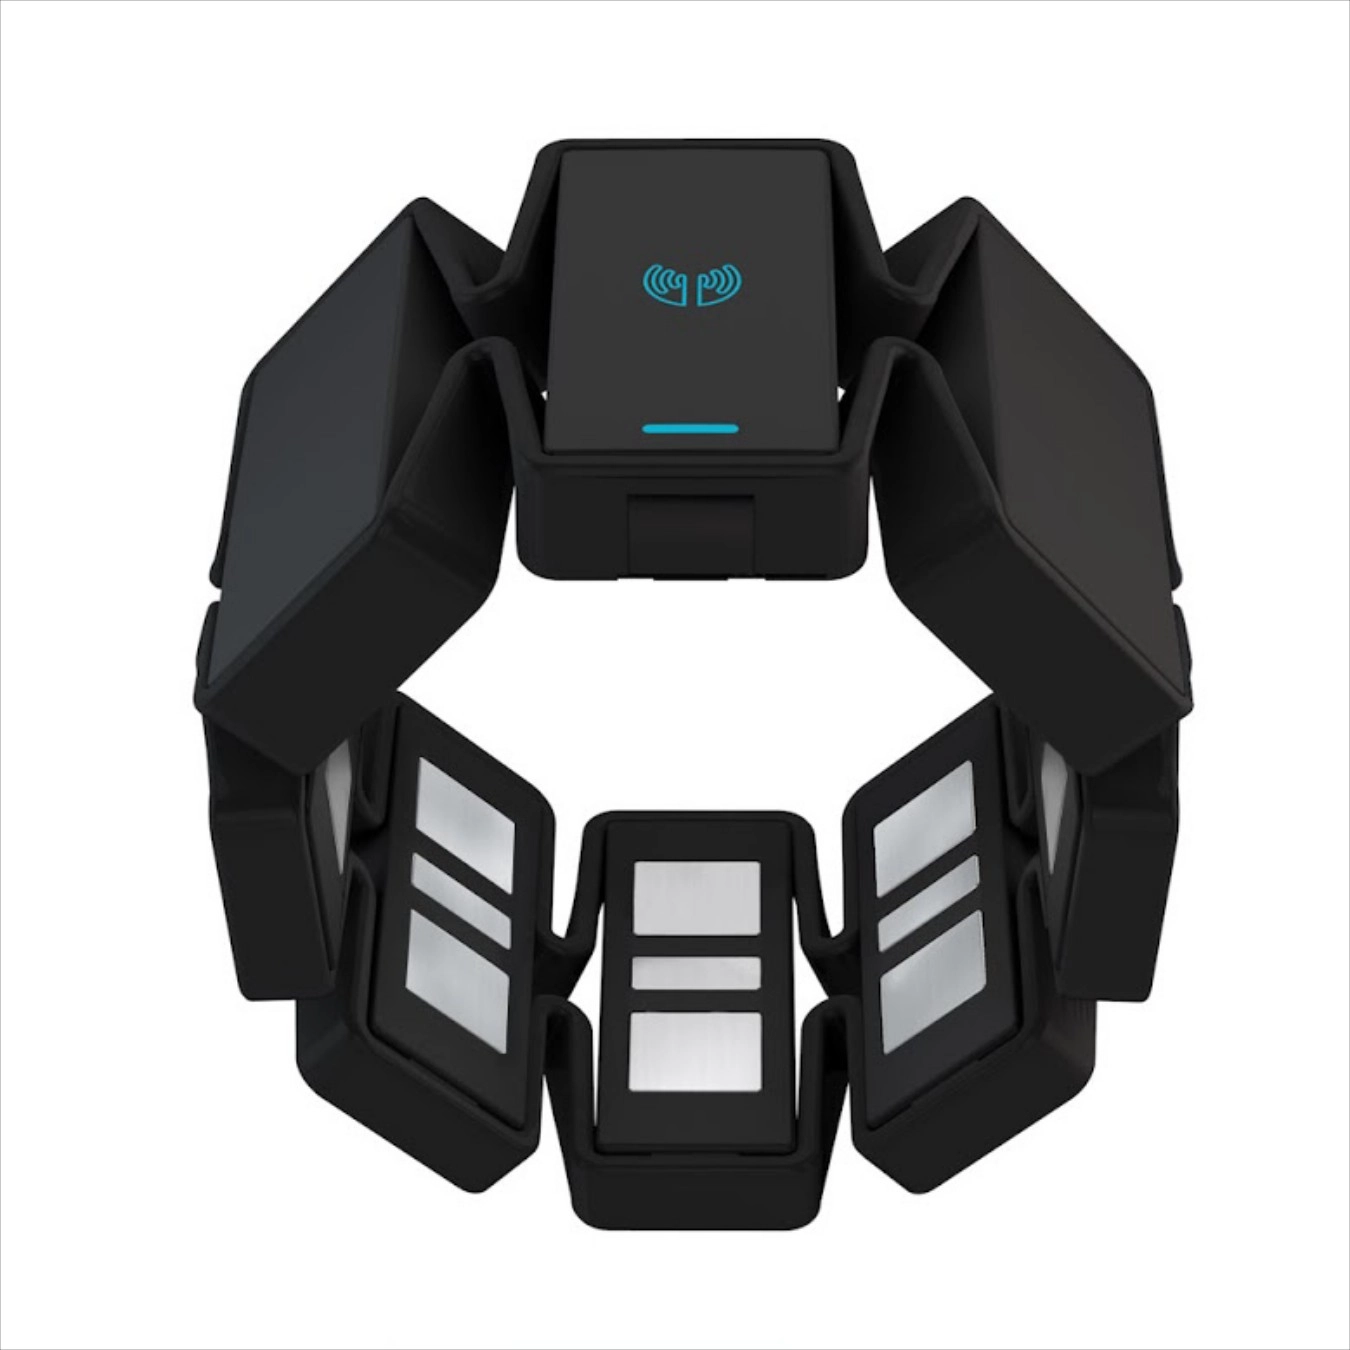
\includegraphics[width=10cm]{images/myoArmBand.png}
    \caption{Picture of the Myo Armband with 8 sEMG sensors \cite{ref:myoArmBand}}
    \label{fig:myoArmband}
\end{figure}

 In 2021, this device is not available in the market anymore. However, a new patent from \textit{Facebook}, release on the 2nd of February 2021 and called \textit{CAMERA - GUIDED INTERPRETATION OF NEUROMUSCULAR SIGNALS } \cite{ref:facebookPatent}, which describes a work similar to this document, shows an improved version of the armband with 16 electrodes. Thus, we can expect similar devices to be released in the market again in the future.



\subsection{Gestures performed}

To create a data set that enables regression models of the finger kinematics, we need a set of gestures that is as big as possible and allows to distinguish the muscular activity linked to each finger independently even if they do not reflect real life movements. This task is difficult as each gesture involves similar sets of muscles.
The needed gestures are also different than for classification model where the set of gestures only need to be as small as possible and to only contain real life movements.


\subsubsection{Single finger motions}

The simplest set of gesture to estimate simultaneously each finger kinematics is composed only of single finger gestures. That is, flexion and extension of one finger at a time with maximum amplitude. 

This techniques has been used in multiple studies \cite{ref:singleFingerGestPlusSignLang, ref:singleFingerGest1, ref:singleFingerGest2} that tried to create regression and classification model of the finger kinematics. They report to have good prediction accuracy (more than 97.5\% in \cite{ref:singleFingerGestPlusSignLang}) but only share the result of the estimation of single finger gestures. Thus, movements involving more than one fingers might not have a good prediction accuracy.


\subsubsection{Activities of daily living (ADL)}

ADLs are gestures that represents real life movements of everyday life. For example, tying a shoelace or typing on a keypad are considered as ADLs. The advantage of using ADLs as base for an hand gesture regression data set is that they allow to get the mot precision for gestures that the final users will be often performing. The KIN-MUS IJI data set \cite{ref:KinMusUji} based its gestures on 26 ADL. 20 of them are taken from the Sollerman Hand Function test (SHFT), which is often used to evaluate the upper extremity’s functional recovery \cite{doi:SHFT}. These 20 ADL aims at showing similar muscle activation pattern as the eight most common hand grips. Performing ADL gesture involve the subject to interact with objects which must be taken into account for the data collection protocol.


\subsubsection{Sign language}

Studies have tried to create sEMG based devices capable of translating sign language into text \cite{ref:signLang, ref:signLang2}. In particular, the Taiwanese sign language is known to contain 50 fundamental postures which involve lots of linkage of multiple fingers \cite{ref:singleFingerGestPlusSignLang, ref:signLang}.

\begin{figure}[H]
    \centering
    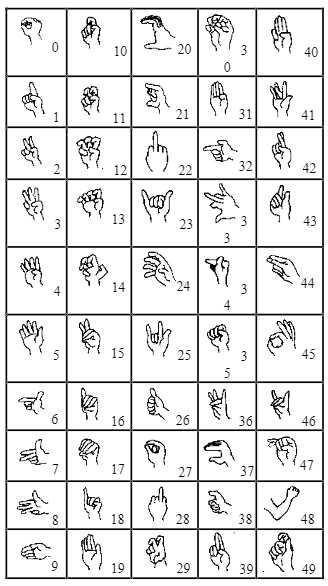
\includegraphics[width=5cm]{images/taiwaneseSignLanguage.png}
    \caption{The 50 fundamental postures of Taiwanese sign language \cite{ref:signLang}}
    \label{fig:signLang}
\end{figure}

Sign languages also has the advantage of giving a set of many postures that are well identifiable from each other. This gives better chance for a classification model to get a high accuracy. It has been shown that, even a small number of sEMG electrodes (organized in a myo armband \cite{ref:myoArmBand}) enable to get classify such gestures with good precision \cite{ref:signLang2}.





\subsubsection{Irregular moves}

A study \cite{ref:Ngeo2014} has used 3 kinds of exercises. The last one was to ask the subject to move its hands freely while keeping a neutral position of the forearm. They encouraged the subject to make irregular gestures in order to get a lot of information on the possible combination of fingers flexion and extension.


\subsubsection{Maximum voluntary contraction (MVC)}
https://jneuroengrehab.biomedcentral.com/articles/10.1186/1743-0003-11-122

https://pubmed.ncbi.nlm.nih.gov/29355119/


The recording of maximum voluntary contractions allow to find the maximum amplitude of the EMG signals which can be later used to normalize the signals.
There are height different postures of the hand for which a MVC can be recorded (see figure \ref{fig:mvc}).

\begin{figure}
    \centering
    \includegraphics[width=10cm]{images/mvc.png}
    \caption{Representations of the 8 postures of the hand for which a MVC can be recorded}
    \label{fig:mvc}
\end{figure}

Studies creating synchronized hand kinematics and sEMG data sets have included this kind of recording in their data \cite{ref:Ngeo2014, ref:KinMusUji} but they do not include the 8 possible postures. Their protocol of data collection for MVC was composed of a few records (i.e. 3 records of each MVC) with 3 minutes of resting between each repetition of the set of postures due to the muscle fatigue that it causes, which can lead to less accurate data.


\subsection{Hand position data representation}

\subsubsection{Gesture duration and repetition}


\subsection{Synchronization}




\section{Motion tracking using the Oculus Quest}


The techniques of motions captures presented in section \ref{sec:motionCaptureTech} have the disadvantage to be expensive and difficult to use. The 3D motion camera tracking system using marker is even criticized as been unreliable for hand motion tracking. In order to propose a data collection benchmark that is reliable and easily reproducible, we present the use of a different device that is able to perform hand tracking quickly and for a reasonable amount of money.

The Oculus Quest is a virtual reality headset developed by Facebook (\url{https://www.oculus.com/quest/}). It has 4 infra-red mounted cameras which are oriented to film the user hands from different angles. The headset is then able to reconstruct in real time a pair of 3D hands which accurately match the user gestures. The pose reconstruction technique is similar different from a conventional motion tracking system as it does not need any marker on the subject. It relies on a deep neural network which only takes to camera vision as input and uses an architechture similar to PoseNets; a model from TensorFlow used for human posture estimation (\url{https://www.tensorflow.org/lite/examples/pose_estimation/overview}) \cite{ref:oculus1, ref:oculus2}.

\subsubsection{Advantages of the Oculus Quest device}
\begin{itemize}
    \item It is cheap compared to the others (399 euros)
    \item It can estimate 26 degrees of freedom for each hand \cite{ref:oculus2}
    \item The neural network is specifically trained to estimate hand gesture which allows more accurate estimation than conventional motion tracking
     \url{https://developer.oculus.com/documentation/unity/unity-utilities-overview/})
    \item It is fast to setup for data collection
    \item It can be controlled remotely using a USB-c cable
    \item A programming library is available to easily use it (OVR library for the Unity game engine
    \item The programming library provides additional pieces of information like the quality of the estimation for each finger and a pinching boolean that tells if a given finger is touching the thumb of the same hand.
\end{itemize}

\subsubsection{Disadvantages of the Oculus Quest device}
\begin{itemize}
    \item The precision of the estimation is not the same for all fingers
    \item If a single joint is incorrectly predicted, it can cause big prediction errors \cite{ref:oculus1}
    \item If the background color is similar to the skin color, the estimation becomes less accurate \cite{ref:oculus1}
    \item There is no documentation on the accuracy of the estimation. We can only rely on testers feeling about it \cite{ref:oculus3}
    \item Its sampling rate is quite low (50 or 60Hz depending on the electrical frequency in the country)
\end{itemize}


\subsubsection{Unity}

In order to collect the data of the gesture estimation from the Oculus Quest, we need to use the Unity game engine (\url{https://unity.com/}). It is a really easy to use framework that enables to build 3D scenes and can be programmed in $C\#$. It has a lot of documentation, receives regular update since 2005 and has a huge community of developers. There also exist an asset store which enables to download lots of assets to put in the built software.\cite{ref:oculus4}

\paragraph{The OVR library}

To use the Oculus quest components from a Unity project, we need to use the Unity OVR library (\url{https://developer.oculus.com/documentation/unity/unity-utilities-overview/}) which provides all the classes that allows to use the hand tracking option of the headset and to collect its data. When it is setup, the user is able to see its hands in the virtual reality and to program can get, at each frame (50 frames per seconds), the rotation of each bone of the 2 hands as well as the additional information provided by the library.

\begin{figure}[h]
    \centering
    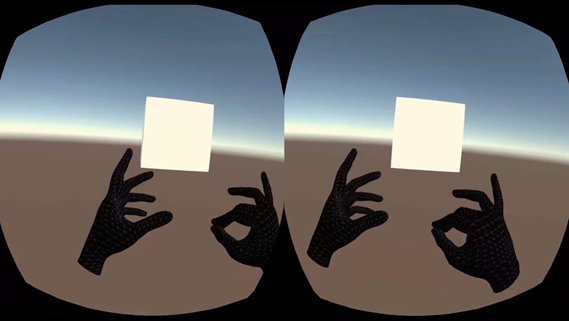
\includegraphics[width=10cm]{images/questView.png}
    \caption{View of the estimated hands from the Oculus quest Virtual Reality headset}
    \label{fig:cyberGlove3}
\end{figure}

The information that can be collected for each hand and at each frame from the headset is:
\begin{enumerate}
    \item The position and rotation of the hand in the 3D space
    \item The 3D rotation of 17 bones of the hand
    \item A boolean telling if the estimation could be processed (false means that the neural network failed to predict the pose)
    \item A boolean per finger indicating if the quality of the estimation of its pose is high or low
    \item A boolean per finger, except the thumb, indicating if it is touching the thumb of the same hand (pinching)
\end{enumerate}
The device is also able to compute the UTC timestamps of each frame which can b used for synchronization.

\paragraph{The Hand Tracking Gesture Recorder library}

The OVR library can be completed with a hand gesture data collection library (\url{https://github.com/jorgejgnz/HandTrackingGestureRecorder}). Made by Jorge Juan González (HCI Researcher at I3A (UCLM)), it enables to record a pose of the hand using the Oculus Quest so that that, later, the program produces a trigger when the user does the same pose. It is possible to save multiple gestures in a file and load them when starting the program on the headset.

This library takes as input all the bones of the hand and tries, based on their relative position to the wrist, to find the pose, among the recorded ones, that is the more probable to be the current pose. If no pose has a high enough probability, it does not output any prediction.



\part{Realisation: Creation of a synchronized EMG/EEG/hand-gesture data set}


\section{Experimental setup}

\begin{figure}[H]
    \centering
    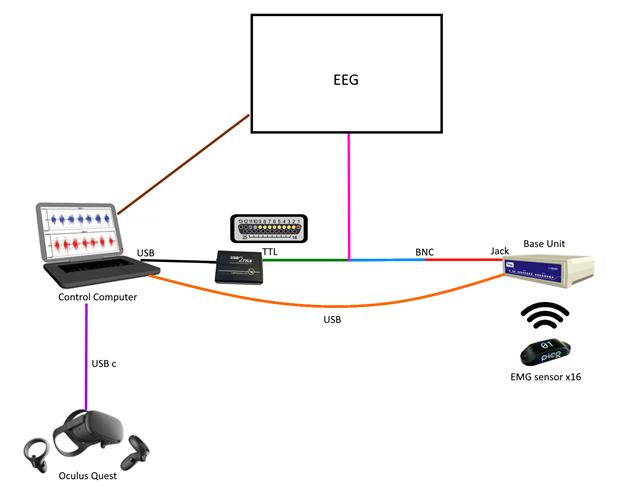
\includegraphics[width=10cm]{images/experimentalSetup.png}
    \caption{Diagram of the experimental setup for data collection}
    \label{fig:experimentalSetup}
\end{figure}


\section{Hand gesture data collection from the Oculus Quest}

In this section, we describe the development of a Unity project that can be executed on the Oculus Quest headset to collect hand motion data. The first part of this software is the setup of the OVR library in a new Unity 3D project. When this project is built in an APK file and loaded on the Oculus Quest, it can already display the user hands using motion tracking.

\subsection{Data collection}

A $C\#$ script called $dataSaving.cs$ is placed in the Unity scene to record all the information of the motion tracking. This script has a function $FixedUpdate()$ which is called by the engine with a regular period (set to a frequency of 50Hz to match the motion tracking frequency). This function has access to the scripts $OVRSkeleton$ and $OVRHand$ of both hands which contain the information on a current hand gesture. It can also get the variable $System.DateTime.UtcNow.Ticks$ to get the UTC of the frame, which will be later used for synchronization.

All the collected data is appended in a csv file (with $";"$ separator) where each line represent a single frame. A description of this file is given below.

\begin{table}[H]
    \centering
    \begin{tabular}{|c|p{12cm}|}
        \hline
        Column index & data \\
        \hline
        1 & UTC \\ \hline
        2 & Boolean telling if the whole data of the left hand is valid \\ \hline
        3 & Position (x, y, z) and rotation (x, y, z) of the left hand in the 3D space \\ \hline
        4 - 22 & Rotation (x, y, z) of 19 bones of the left hand \\ \hline
        23 - 26 & Boolean telling if the fingers 2 to 5 of the left hand are touching the thumb of the left hand (pinching action) \\ \hline
        27 - 31 & Boolean telling if the confidence in the quality of the pose estimation of the finger 1 to 5 is high or low \\ \hline
        32 - 61 & Same as 2 - 31 but for the right hand \\ \hline
        62 & Name of the gesture recognized by the library \textit{Hand Tracking Gesture  Recorder} (\url{https://github.com/jorgejgnz/HandTrackingGestureRecorder}) among those recorded for the right hand\\
        \hline
    \end{tabular}
    \caption{Caption}
    \label{tab:my_label}
\end{table}

The indexes of the fingers are:
\begin{enumerate}
    \item Thumb
    \item Index
    \item Middle
    \item Ring
    \item Pinky
\end{enumerate}

The indexed of each finger bone can be found in the documentation of the OVR library (\url{https://developer.oculus.com/documentation/unity/unity-handtracking/}) and is described in figure \ref{fig:ovrHandIndexesTab} and shown in figure \ref{fig:ovrHandIndexes}.

\begin{figure}[h]
    \centering
    \begin{verbatim}
Hand_WristRoot   = Hand_Start + 0 // root frame of the hand, where the wrist is located
Hand_ForearmStub = Hand_Start + 1 // frame for user's forearm
Hand_Thumb0      = Hand_Start + 2 // thumb trapezium bone
Hand_Thumb1      = Hand_Start + 3 // thumb metacarpal bone
Hand_Thumb2      = Hand_Start + 4 // thumb proximal phalange bone
Hand_Thumb3      = Hand_Start + 5 // thumb distal phalange bone
Hand_Index1      = Hand_Start + 6 // index proximal phalange bone
Hand_Index2      = Hand_Start + 7 // index intermediate phalange bone
Hand_Index3      = Hand_Start + 8 // index distal phalange bone
Hand_Middle1     = Hand_Start + 9 // middle proximal phalange bone
Hand_Middle2     = Hand_Start + 10 // middle intermediate phalange bone
Hand_Middle3     = Hand_Start + 11 // middle distal phalange bone
Hand_Ring1       = Hand_Start + 12 // ring proximal phalange bone
Hand_Ring2       = Hand_Start + 13 // ring intermediate phalange bone
Hand_Ring3       = Hand_Start + 14 // ring distal phalange bone
Hand_Pinky0      = Hand_Start + 15 // pinky metacarpal bone
Hand_Pinky1      = Hand_Start + 16 // pinky proximal phalange bone
Hand_Pinky2      = Hand_Start + 17 // pinky intermediate phalange bone
Hand_Pinky3      = Hand_Start + 18 // pinky distal phalange bone
\end{verbatim}
    \caption{Indexes of the ones of the OVR hand as given by the OVR library}
    \label{fig:ovrHandIndexesTab}
\end{figure}

\begin{figure}[H]
    \centering
    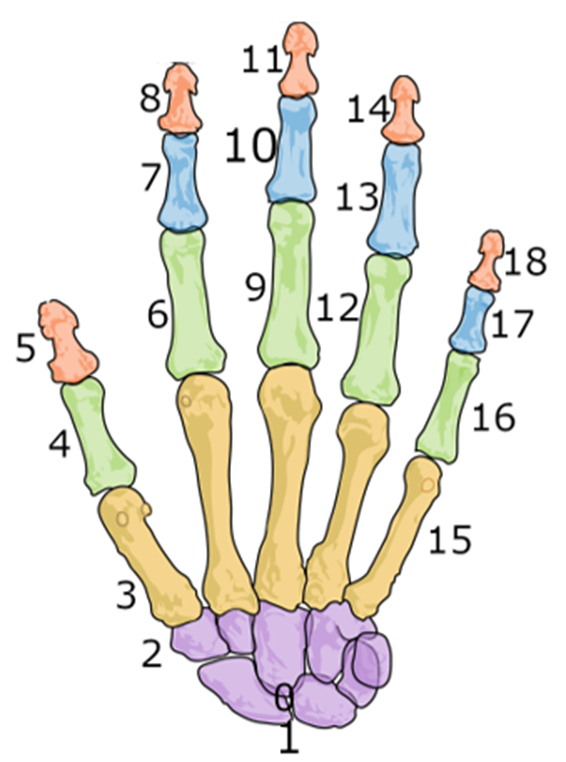
\includegraphics[width=7cm]{images/ovrHandBonesIndexes.png}
    \caption{Graphical representation of the indexes of the ones of the OVR hand as given by the OVR library (\url{https://www.reddit.com/r/OculusQuest/comments/edkp9i/visual_reference_for_hand_tracking_bone_ids/})}
    \label{fig:ovrHandIndexes}
\end{figure}

This is saved in a local file on the Oculus Quest and can be exported to an external computer after the recording using an USB-c link.


\subsection{Remote control}

The experimental setup is made so that the subject does not have to do anything else than the recorded hand gestures. In order to do that, a remote control interface was implemented. It enables to send messages to the Unity program running on the Oculus Quest from an external computer using a USB-c link. Theses messages take the form of files that are pushed in a particular directory, and with a name giving to the action to perform, using \textit{Android Debug Bridge} (ADB: \url{https://developer.android.com/studio/command-line/adb}).

A python script called $remoteControl.py$ was implemented to give an interface to remotely control the Oculus Quest behaviour. The actions that can be done are
\begin{itemize}
    \item Start and stop the recording of the hand motion. A sphere in the 3D Unity scene, seen from the Oculus Quest, changes color to indicate if the recording is activated (red=off, green=on). Stopping the recording also pulls the record file on the computer running this script.
    \item Reset the recording
    \item Save the current gesture of the right hand for the Hand Tracking Gesture  Recorder library
    \item Export the saved right hand gesture in a file (local on the Oculus Quest)
    \item Import the right hand gesture from a file (local on the external computer)
    \item Show the next instruction to the user (described later in the document)
\end{itemize}

\subsection{Interface}




\section{Data synchronization}

An important point of the data set creation is the synchronization of the hand kinematics with the EMG and EEG signals. To perform this synchronization, we make three assumptions on the setup.
\begin{enumerate}
    \item The recording of the EMG and EEG can be started using a trigger signal with a known delay
    \item The timestamps given by the EMG, EEG
    \item The UTC of the external computer and those of the Oculus Quest are synchronized
\end{enumerate}
The 2 first assumptions are relying on the official user manuals of the hardware. We know that the Cometa EMG has a starting delay of 14ms when using a triggered start. The delay for the EEG is \color{red} [TO FIND] \color{black}. The EEG cannot be started with a trigger but it can include the trigger timestamp in its recorded data. So, we just have to cut the data before the first trigger.

To verify the third assumption, we can use the software \textit{SideQuest} (\url{https://sidequestvr.com/}) that enables to stream the screen of the Oculus Quest on a computer using a USB-c cable (called Oculus Link). By doing so, we find a shift of approximately 22ms in average with a standart deviation around 100ms between the computers UTC and the Oculus Quests UTC. This time lag corresponds to the known delay of the SideQuest streaming (\url{https://www.mdpi.com/2073-431X/9/4/92}) which allows us to conclude that they are synchronized.

The algorithm to synchronize the data from the external computer is the following:
\begin{enumerate}
    \item Start the hand motion recording (which takes unknown time) and EEG recording
    \item Wait for the Oculus Quest to send a feedback that its recording has started
    \item Save the current UTC
    \item Send a trigger start signal on the EMG recorder and the EEG recorder
    \item Collect the data until the end of the recording
    \item stop all recording (they might not end exactly at the same time but the timestamps in each part of the records removes the need for synchronized end of record)
    \item Cut the start of the hand kinematics recording at the UTC of the starting of the EMG/EEG recording
    \item Convert the UTC in the hand kinematic file to timestamps in ms starting from 0 (0 corresponds to the UTC saved at the beginning of the recording but there might not be a recorded frame at this exact moment)
    \item Shift the EMG recording by 14ms
    \item Shift the EEG recording by \color{red} [TO FIND] \color{black}
    \item Cut the beginning of the EEG recording (before the first trigger)
    \item place everything in a common folder
\end{enumerate}



\section{Data collection protocol}

\subsection{Placement of the sEMG electrodes}

\subsection{Gestures to perform}



\part{Conclusion and future work}


\bibliographystyle{plain}
\bibliography{biblio}
\cite{*}


\end{document}
